
\documentclass[12pt]{article}

\usepackage[utf8]{inputenc}
\usepackage[greek, english]{babel}

% Packages
\usepackage{MnSymbol}
\usepackage{alphabeta}
\usepackage{amsfonts}
\usepackage{amsmath}
\usepackage{amsthm}
\usepackage{caption}
\usepackage{graphicx}
\usepackage{latexsym}
\usepackage{stackrel}
\usepackage{titlesec}

% Commands
\newcommand{\R}{\mathbb{R}}
\newcommand{\N}{\mathbb{N}}
\newcommand{\norm}[1]{\left\lVert#1\right\rVert}
\newcommand{\margin}{\hspace{4pt}}
\newcommand{\centered}[1]{\begin{align*}#1\end{align*}}
\newcommand{\plot}{\includegraphics}

% Environments
\newenvironment{rcases}
	{\left.\begin{aligned}}
	{\end{aligned}\right\rbrace}

\newenvironment{matlab}
	{\begin{figure}[hp]\centering\captionsetup{justification=centering}}
	{\end{figure}}

\setlength{\parindent}{0in}
\setlength{\oddsidemargin}{0in}
\setlength{\textwidth}{6.5in}
\setlength{\textheight}{10in}
\setlength{\topmargin}{-1.0in}
\setlength{\headheight}{18pt}

\titlespacing*{\subsection}
{0pt}{5.5ex plus 1ex minus .2ex}{4.3ex plus .2ex}

\title{\hugeΑλγοριθμική Επιχειρησιακή Έρευνα\\Δεύτερη Εργασία}
\author{Σιώρος Βασίλειος\\Ανδρινοπούλου Χριστίνα}
\date{Οκτώβριος 2019}

\begin{document}

\maketitle

\pagenumbering{gobble}

\pagebreak


\subsection*{1. Find a differentiable function \( f: \R \rightarrow \R \) such that f does not have an extremum at its
critical point.}

Έστω η συνάρτηση \( f(x) = x^3 : \R \rightarrow \R \), η οποία είναι γνωστό ότι είναι
παραγωγίσιμη στο \( \R \). στο σημείο λόγους σαφήνειας, θα αποδείξουμε τη συνέχεια και την παραγωγισιμότητα της
στο \( x = 0 \). \\

\( \bullet \) \textbf{Συνέχεια:} \\

\begin{align*}
    &\begin{rcases}
        \lim_{x \to 0^-} f(x) & = \lim_{x \to 0^-} x^3 & = 0 \\
        \lim_{x \to 0^+} f(x) & = \lim_{x \to 0^+} x^3 & = 0
    \end{rcases}
    \Rightarrow \\
    &\lim_{x \to 0} f(x) = 0
\end{align*}

\begin{align*}
    &\begin{rcases}
        f(0) = 0^3 & = 0 \\
        \lim_{x \to 0} f(x) & = 0
    \end{rcases}
    \Rightarrow \\
    &f(0) = \lim_{x \to 0} f(x)
\end{align*}

\( \bullet \) \textbf{Παραγωγισιμότητα:} \\

\begin{align*}
    &\begin{rcases}
        \lim_{x \to 0^-} \frac{f(x) - f(0)}{x - 0} &= \lim_{x \to 0^-} \frac{x^3}{x} &= \lim_{x \to 0^-} x^2 &= 0 \\
        \lim_{x \to 0^+} \frac{f(x) - f(0)}{x - 0} &= \lim_{x \to 0^+} \frac{x^3}{x} &= \lim_{x \to 0^+} x^2 &= 0
    \end{rcases}
    \Rightarrow \\
    &\lim_{x \to 0} \frac{f(x) - f(0)}{x - 0} = 0
\end{align*} \\

Επομένως, δείξαμε ότι η συνάρτηση \( f(x) = x^3 \) είναι συνεχής και παραγωγίσιμη στο σημείο \( x = 0 \). \\

Το σημείο \( x = 0 \) αποτελεί κρίσιμο σημείο της \(f\), αφού η παράγωγός της μηδενίζεται εκεί.
Ωστόσο, όπως φαίνεται και από την ακόλουθη γραφική παράσταση, το σημείο \( x = 0 \)  δεν αποτελεί ακρότατο της. \\

\pagebreak

\begin{matlab}
    \plot{cubic_figure}
    \caption{An example of a differentiable function \( f: \R \rightarrow \R \) which does not have an extremum at its critical point}
\end{matlab}

\vspace{2in}

\pagebreak

\subsection*{2. Given a positive integer \( S \), which decompositions
\centered{a_1 + \dotsb + a_n = S}
with the \( a_i \) positive integers have the largest product \( a_1 \cdot \dotsb \cdot a_n \)?}

Αρχικά, μοντελοποιήσαμε το πρόβλημα, με στόχο να αναδείξουμε κάποιο πιθανό μοτίβο. \\

Παρατίθονται τα ευρήματα μας, όσον αφορά ακέραιες τιμές στο διάστημα \( \lbrack 10, \margin 20 \rbrack \). \\

\centered{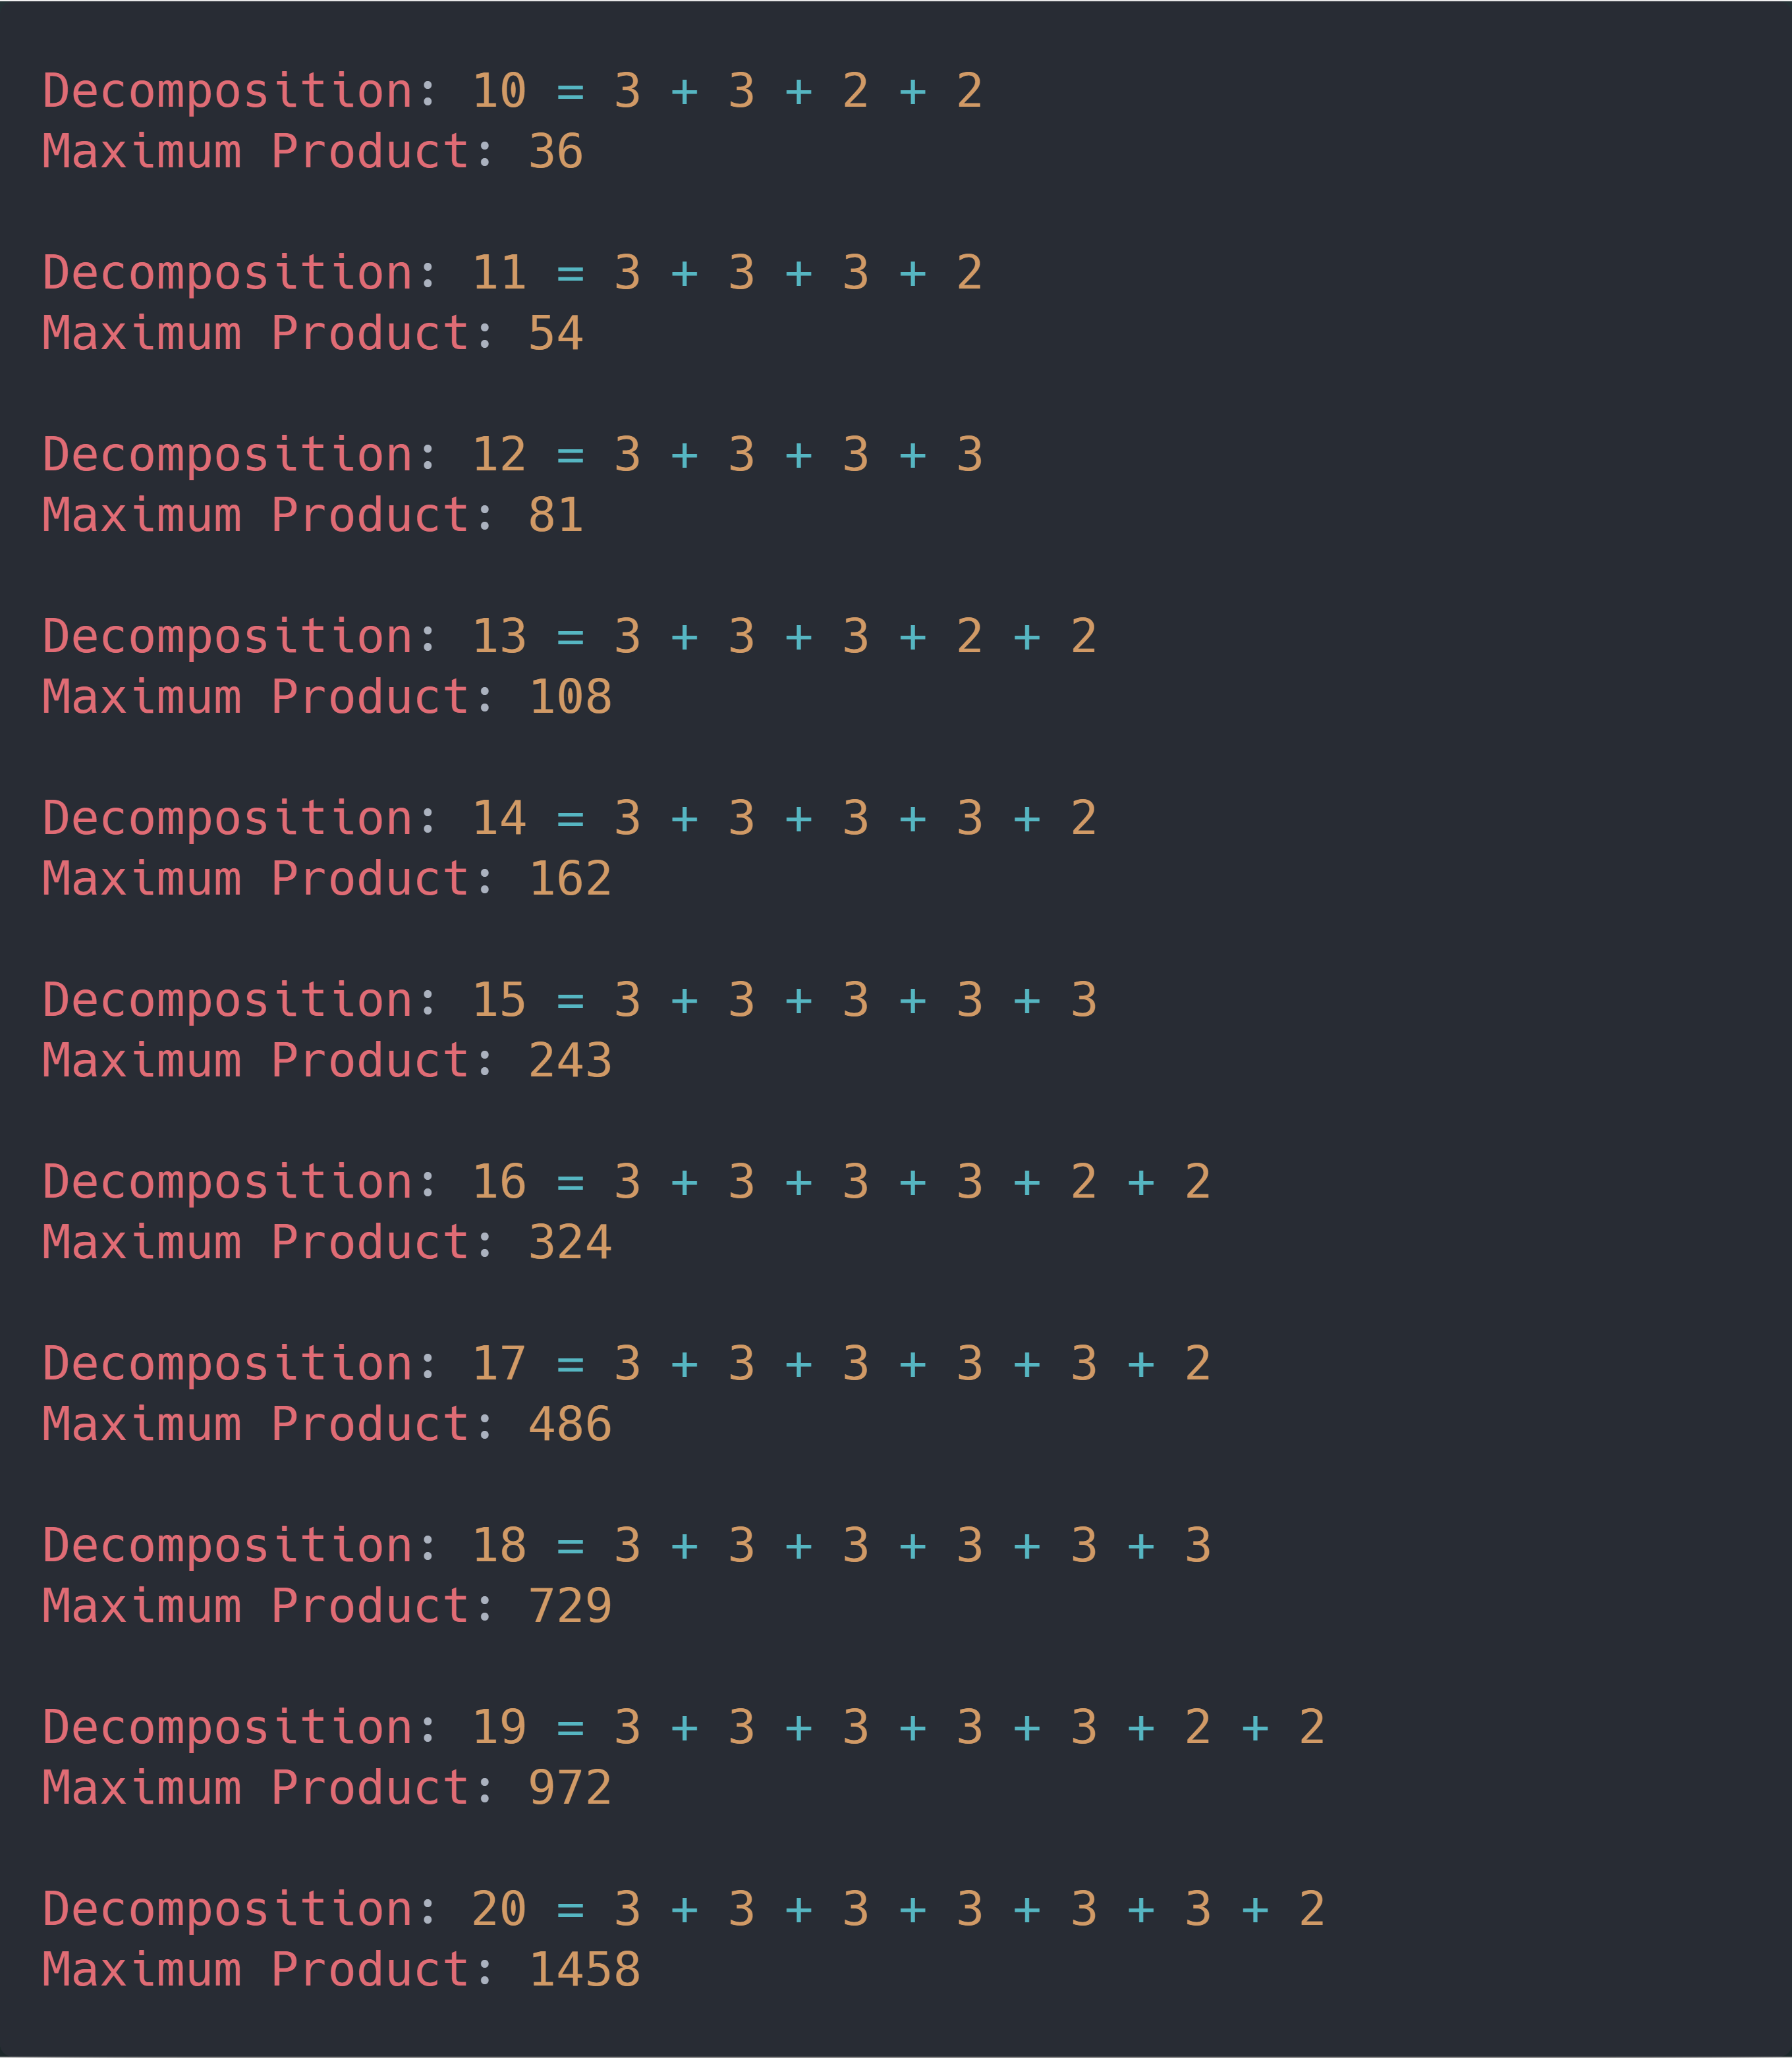
\includegraphics[scale=0.171875]{partition_output.png}} \\

Παρατηρούμε πως, σε κάθε περίπτωση, η αποδόμηση του εκάστοτε αριθμού με το μέγιστο γινόμενο αποτελείται αποκλειστικά από 3 και 2. \\

Θεωρούμε τυχαίο θετικό ακέραιο \( S \) και την αποδόμησή του \\

\centered{S = a_1 + \dotsb + a_n}

με το μέγιστο γινόμενο \\

\centered{\stackrel{max}{\prod} = \prod_{i = 1}^{n} a_i}

Έστω ότι υπάρχει \( 1 \leq k \leq n \) τέτοιο ώστε \( a_k \geq 4 \).
Διακρίνουμε τις εξής περιπτώσεις: \\

\( \bullet \) \( a_k = 2 \cdot l \margin \mid \margin l \in \N^+ \) \\

Δεδομένου ότι \( a_k \geq 4 \), έχουμε

\begin{align*}
    &\begin{rcases}
        a_k & & \geq 4 & \Leftrightarrow a_k & \geq 0 \\
        a_k & & \geq 4 & \Leftrightarrow a_k - 4 & \geq 0
    \end{rcases}
    \stackrel{\times}{\Rightarrow} \\
    &a_k \cdot (a_k - 4) \geq 0 && \Leftrightarrow \\
    &a_k^2 - 4 \cdot a_k \geq 0 && \Leftrightarrow \\
    &a_k^2 \geq 4 \cdot a_k && \Leftrightarrow \\
    &\frac{a_k^2}{4} \geq a_k
\end{align*}

Δεδομένου ότι

\centered{a_k = 2 \cdot l \margin \mid \margin l \in \N^+ \Leftrightarrow a_k \in N^+}

μπορούμε να ορίσουμε μια νέα αποδόμηση του \( S \), ως εξής

\centered{S = a_1 + \dotsb + \frac{a_k}{2} + \frac{a_k}{2} + \dotsb + a_n}

Το γινόμενο της παραπάνω αποδόμησης είναι

\begin{align*}
    \prod_{i = 1}^{n} a_i & = a_1 \times \dotsb \times \frac{a_k}{2} \times \frac{a_k}{2} \times \dotsb \times a_n && \Leftrightarrow \\
    \prod_{i = 1}^{n} a_i & = a_1 \times \dotsb \times \frac{a_k^2}{4} \times \dotsb \times a_n && \Leftrightarrow \\
    \prod_{i = 1}^{n} a_i & \geq a_1 \times \dotsb \times a_k \times \dotsb \times a_n && \Leftrightarrow \\
    \prod_{i = 1}^{n} a_i & \geq \stackrel{max}{\prod}
\end{align*}

Το παραπάνω αποτέλεσμα είναι αδύνατον, αφού υποθέσαμε πως \( \stackrel{max}{\prod} \) είναι η αποδόμηση του θετικού ακεραίου
\( S \) με το μέγιστο γινόμενο. Καταλήξαμε δηλαδή σε άτοπο, γεγονός που συνεπάγεται ότι η υπόθεση μας ήταν λανθασμένη. \\

Ως εκ τούτου δεν υπάρχει \( 1 \leq k \leq n \) τέτοιο ώστε \( a_k \geq 4 \). \\

\( \bullet \) \( a_k = 2 \cdot l + 1 \margin \mid \margin l \in \N \) \\

Δεδομένου ότι \( a_k \geq 4 \), έχουμε

\centered{a_k = 2 \cdot l + 1 \geq 4 \Leftrightarrow l \geq 2}

και άρα

\begin{align*}
    &\begin{rcases}
        l & \geq 2 & \Leftrightarrow l & \geq 1 \\
        l & \geq 2 & \Leftrightarrow l - 1 & \geq 1 \\
    \end{rcases}
    \stackrel{\times}{\Rightarrow} \\
    &l \cdot (l - 1) & \geq 1 && \Leftrightarrow \\
    &l^2 - l & \geq 1 && \Leftrightarrow \\
    &l^2 - l + 2 \cdot l & \geq 1 + 2 \cdot l && \Leftrightarrow \\
    &l^2 + l & \geq 1 + 2 \cdot l && \Leftrightarrow \\
    &l \cdot (l + 1) & \geq 2 \cdot l + 1 && \Leftrightarrow \\
    &l \cdot (l + 1) & \geq a_k
\end{align*}

Δεδομένου ότι

\centered{l \in \N \cap l \geq 2 \Leftrightarrow l \in N^+}

μπορούμε να ορίσουμε μια νέα αποδόμηση του \( S \), ως εξής

\centered{S = a_1 + \dotsb + l + (l + 1) + \dotsb + a_n}

Το γινόμενο της παραπάνω αποδόμησης είναι

\begin{align*}
    \prod_{i = 1}^{n} a_i & = a_1 \times \dotsb \times l \times (l \times 1) \times \dotsb \times a_n && \Leftrightarrow \\
    \prod_{i = 1}^{n} a_i & \geq a_1 \times \dotsb \times a_k \times \dotsb \times a_n && \Leftrightarrow \\
    \prod_{i = 1}^{n} a_i & \geq \stackrel{max}{\prod}
\end{align*}

Το παραπάνω αποτέλεσμα είναι αδύνατον, αφού υποθέσαμε πως \( \stackrel{max}{\prod} \) είναι η αποδόμηση του θετικού ακεραίου
\( S \) με το μέγιστο γινόμενο. Καταλήξαμε δηλαδή σε άτοπο, γεγονός που συνεπάγεται ότι η υπόθεση μας ήταν λανθασμένη. \\

Ως εκ τούτου δεν υπάρχει \( 1 \leq k \leq n \) τέτοιο ώστε \( a_k \geq 4 \). \\

\pagebreak

Η μονάδα, όντας το ουδέτερο στοιχείου το πολλαπλασιασμού, δεν συνεισφέρει θετικά στο τελικό γινόμενο καμίας αποδόμησης
που την εμπεριέχει κι ως εκ τουτου δεν θα εμφανίζεται σε καμία αποδόμηση μεγίστου γινομένου, πλην τετριμμένων περιπτώσεων. \\

Από τα πειράματα μας παρατηρούμε πως, ο αριθμός 2 δεν εμφανίζεται παραπάνω από 2 φορές σε καμία αποδόμηση μεγίσου γινομένου. \\

Αυτό είναι λογικό καθώς, δεδομένης μίας αποδόμησης του θετικού ακεραίου \( S \) της μορφής

\centered{S = a_1 + \dotsb + 2 + 2 + 2 + \dotsb + a_n}

μπορούμε να ορίσουμε μία νέα αποδόμηση

\centered{S = a_1 + \dotsb + 3 + 3 + \dotsb + a_n}

της οποίας το γινόμενο είναι

\begin{align*}
    \prod_{i = 1}^{n} a_i & = a_1 \times \dotsb \times 3 \times 3 \times \dotsb \times a_n && \Leftrightarrow \\
    \prod_{i = 1}^{n} a_i & = a_1 \times \dotsb \times 9 \times \dotsb \times a_n && \Leftrightarrow \\
    \prod_{i = 1}^{n} a_i & \geq a_1 \times \dotsb \times 8 \times \dotsb \times a_n && \Leftrightarrow \\
    \prod_{i = 1}^{n} a_i & \geq a_1 \times \dotsb \times 2 \times 2 \times 2 \times \dotsb \times a_n
\end{align*}

Έτσι η αποδόμηση μεγίστου γινομένου δίνεται από τη σχέση

\centered{S = 3 \cdot x + 2 \cdot \frac{S - 3 \cdot x}{2}}

και το γινόμενο της από τη σχέση

\centered{\stackrel{max}{\prod} = 3^x \times 2^{\frac{S - 3 \cdot x}{2}}}

\vspace{2in}

\pagebreak

\subsection*{3. Find the optimal solution to the Diet Problem when the cost function is
\centered{Cost(x_1, x_2) = x_1 + x_2 \text{.}}}

Οι περιορισμοί μας είναι οι εξής

\begin{align*}
    30 \cdot x_1 + 5 \cdot x_2 & \geq 60 \\
    15 \cdot x_1 + 10 \cdot x_2 & \geq 70 \\
    x_1, x_2 & \geq 0
\end{align*}

και επιθυμούμε να ελαχιστοποιήσουμε τη συνάρτηση

\centered{Cost(x_1, x_2) = x_1 + x_2}

\begin{matlab}
    \plot{diet_problem_figure}
    \caption{The Optimal Solution to the Diet Problem when the total cost is given by the function \( Cost(x_1, x_2) = x_1 \cdot x_2 \)}
\end{matlab}

\pagebreak

Παρατηρούμε ότι, δεν ορίζεται ευθεία, η οποία αντιστοιχεί σε κόστος χαμηλότερο του \textbf{4.67}, τέτοια ώστε,
έστω και ένα σημείο της να πληροί κάθε περιορισμό. Ως εκ τούτου το σημείο τομής των ευθειών

\begin{align*}
    15 \cdot x_1 + 10 \cdot x_2 & = 70 \\
    x_2 & = 0
\end{align*}

δηλαδή το σημείο \textbf{(4.67, 0)}, αποτελεί τη βέλτιστη λύση.

\vspace{2in}

\pagebreak

\subsection*{4. Let A,B $\R^{n\times n}$. Show that the traditional way of computing their product AB requires
a total of $(2n-1)n^2$ arithmetic operations.}

Οι πίνακες Α και Β είναι τετραγωνικοί $(n\times n)$, δηλαδή αποτελόυνται από n γραμμές και από n στήλες, όπως φαίνεται παρακάτω: \\
$$A = \begin{bmatrix}
a_{11} & a_{22} & . . . . & a_{1n} \\
a_{21} & a_{22} & . . . . & a_{2n} \\
. & . & . . . . & . \\
a_{n1} & a_{n2} & . . . . & a_{nn}
\end{bmatrix}$$
$$B = \begin{bmatrix}
b_{11} & b_{22} & . . . . & b_{1n} \\
b_{21} & b_{22} & . . . . & b_{2n} \\
. & . & . . . . & . \\
b_{n1} & b_{n2} & . . . . & b_{nn}
\end{bmatrix}$$
\\
$$ Α\times B = 
\begin{bmatrix}
a_{11} & a_{22} & . . . . & a_{1n} \\
a_{21} & a_{22} & . . . . & a_{2n} \\
. & . & . . . . & . \\
a_{n1} & a_{n2} & . . . . & a_{nn}
\end{bmatrix} 
\begin{bmatrix}
b_{11} & b_{22} & . . . . & b_{1n} \\
b_{21} & b_{22} & . . . . & b_{2n} \\
. & . & . . . . & . \\
b_{n1} & b_{n2} & . . . . & b_{nn}
\end{bmatrix} =
\begin{bmatrix}
z_{11} & z_{22} & . . . . & z_{1n} \\
z_{21} & z_{22} & . . . . & z_{2n} \\
. & . & . . . . & . \\
z_{n1} & z_{n2} & . . . . & z_{nn}
\end{bmatrix} = Ζ
$$
\\
Για τον πολλαπλασιασμό των πινάκων Α και Β αρκεί να πολλαπλασιάσουμε την: \\ 
\[
\left.
\raisebox{1pt}[30pt]{\smash{$\begin{array}{r@{}l@{\,}l}
		\mbox{1η γραμμή του Α με την 1η στήλη του Β, για το $z_{11}$ $\rightarrow$ n γινόμενα και (n-1) προσθέσεις} \\
		\mbox{1η γραμμή του Α με την 2η στήλη του Β, για το $z_{12}$ $\rightarrow$ n γινόμενα και (n-1) προσθέσεις} \\
		\\
		\mbox{1η γραμμή του Α με την n στήλη του Β, για το $z_{1n}$ $\rightarrow$ n γινόμενα και (n-1) προσθέσεις} \\
		\end{array}$}}
\right\} n(n + (n-1))
\]
\\
\[
\left.
\raisebox{1pt}[30pt]{\smash{$\begin{array}{r@{}l@{\,}l}
		\mbox{2η γραμμή του Α με την 1η στήλη του Β, για το $z_{21}$ $\rightarrow$ n γινόμενα και (n-1) προσθέσεις} \\
		\mbox{2η γραμμή του Α με την 2η στήλη του Β, για το $z_{22}$ $\rightarrow$ n γινόμενα και (n-1) προσθέσεις} \\
	   	\\
		\mbox{2η γραμμή του Α με την n στήλη του Β, για το $z_{2n}$ $\rightarrow$ n γινόμενα και (n-1) προσθέσεις} \\
		\end{array}$}}
\right\} n(n + (n-1))
\]
\\
$$...$$
$$...$$
$$...$$
\\
\[
\left.
\raisebox{1pt}[30pt]{\smash{$\begin{array}{r@{}l@{\,}l}
		\mbox{n γραμμή του Α με την 1η στήλη του Β, για το $z_{n1}$ $\rightarrow$ n γινόμενα και (n-1) προσθέσεις} \\
		\mbox{n γραμμή του Α με την 2η στήλη του Β, για το $z_{n2}$ $\rightarrow$ n γινόμενα και (n-1) προσθέσεις} \\
		\\
		\mbox{n γραμμή του Α με την n στήλη του Β, για το $z_{nn}$ $\rightarrow$ n γινόμενα και (n-1) προσθέσεις} \\
		\end{array}$}}
\right\} n(n + (n-1))
\]
\\
Η κάθε γραμμή του πίνακα Α πολλαπλασιάζεται με όλες τις στήλες του Β και προκύπτει μία νέα γραμμή στον πίνακα Ζ. Η παραπάνω διαδικασία απαιτεί n(n+(n-1)) αριθμητικές παραστάσεις και επειδή αυτό θα συμβεί n φορές απαιτούνται συνολικά $n^2(n+(n-1)) = n^2(2n-1)$.
\vspace{2in}

\pagebreak

\subsection*{5. Consider the problem of solving a system of n linear equations in n unknowns. Show
that the Gaussian elimination method requires O($n^3$) arithmetic operations in order to either
compute a solution or to decide that no solution exist.}

Η μέθοδος απαλοιφής του Gauss είναι μία μέθοδος για την επίλυση πυκνών γραμμικών συστημάτων, δηλαδή συστημάτων που ο πίνακας των συντελεστών των αγνώστων στοιχείων αποτελείται κυρίως από μη μηδενικά στοιχεία. \\
Πριν προχωρήσουμε στην εύρεση της πολυπλοκότητας της μεθόδου, θα εξηγήσουμε πως δουλεύει η μέθοδος. \\ \\
Στόχος της απαλοιφής του Gauss είναι να λύσουμε ένα γραμμικό σύστημα $Ax = b$, όπου $A\epsilon \R^{n\times n}$, $x\epsilon \R^{n\times 1}$ και $B\epsilon \R^{n\times 1}$. Για να λύσουμε το σύστημα αυτό, η μέθοδος απαλοιφής του Gauss προχωρά σε τριγωνοποίηση του πίνακα A, κι έτσι ο πίνακας γίνεται άνω τριγωνικός, κι έπειτα με προς τα πίσω αντικατάσταση βρίσκουμε τους αγνώστους. \\ \\
Πιο αναλυτικά, έστω ότι βρισκόμαστε στο k-οστό βήμα της μεθόδου (αυτό σημαίνει ότι κοιτάμε την k γραμμή του πίνακα A). Τα βήματα που ακολουθούμε εδώ είναι: \\
1. Βρίσκουμε $(n-k)$ το πλήθος πολλαπλασιαστές m, όπου $m_{ik} = - \frac{a_{ik}}{a_{kk}}$ για $i=k+1,k+2,...,n$. \\
2. Εφαρμόζουμε τον τύπο $a_{ij}^{new} = a_{ij}^{old} + m_{ik}\times a_{kj}^{(k)}$ \\ για $i = k+1, k+2, ...,n$ και $j = k, k+1,...,n$ \\
3. Εφαρμόζουμε τον τύπο $b_{i}^{new} = b_{i}^{old} + m_{ik}\times _{k}^{(k)}$ \\ για $i = k+1, k+2, ...,n$ \\ \\
Για την εύρεση της πολυπλοκότητας θα αναφερθούμε αρχικά στη γενική περίπτωση επίλυσης $l$ το πλήθος γραμμικών συστημάτων με τον ίδιο πίνακα αγνώστων Α. Άλλωστε, η "βαρια" υπολογιστικά εργασία είναι η τριγωνοποίηση του πίνακα Α. Έπειτα θα περάσουμε στην περίπτωση όπου το $l=1$. \\
Έστω πάλι ότι βρισκόμαστε στο k βήμα της μεθόδου:
$$
\begin{bmatrix}
a_{11} & a_{12} & a_{13} & ... & a_{1k} & a_{1,k+1} & ... & a_{1n}\\
& a_{22}  & a_{23}  & ... & a_{2k}  & a_{2,k+1}  & ... & a_{2n} \\
&  & a_{33}  & ... & a_{3k}  & a_{3,k+1}  & ... & a_{3n} \\
&  &  &  & . & . &  & .\\
& 0 &  & \ddots  & . & . &  & .\\
&  &  &  & . & . &  & .\\
&  &  &  & a_{kk}  & a_{k,k+1}  & ... & a_{kn}  \\
&  &  &  & a_{k+1,k}  & a_{k+1,k+1}  & ... & a_{k+1,n} \\
&  &  &  & . & . &  & .\\
& 0 &  &  & . & . &  & .\\
&  &  &  & . & . &  & .\\
&  &  &  & a_{nk}  & a_{n,k+1}  & ... & a_{nn} 
\end{bmatrix} 
\begin{bmatrix}
x_{1}^{(1)} & x_{1}^{(2)} & ... & x_{1}^{(l)}\\
x_{2}^{(1)} & x_{2}^{(2)} & ... & x_{2}^{(l)}\\
x_{3}^{(1)} & x_{3}^{(2)} & ... & x_{3}^{(l)}\\
. & . &  & .\\
. & . &  & .\\
. & . &  & .\\
x_{k}^{(1)} & x_{k}^{(2)} & ... & x_{k}^{(l)}\\
x_{k+1}^{(1)} & x_{k+1}^{(2)} & ... & x_{k+1}^{(l)}\\
. & . &  & .\\
. & . &  & .\\
. & . &  & .\\
x_{n}^{(1)} & x_{n}^{(2)} & ... & x_{n}^{(l)}
\end{bmatrix}  
=
\begin{bmatrix}
b_{1}^{(1)} & b_{1}^{(2)} & ... & b_{1}^{(l)}\\
b_{2}^{(1)} & b_{2}^{(2)} & ... & b_{2}^{(l)}\\
b_{3}^{(1)} & b_{3}^{(2)} & ... & b_{3}^{(l)}\\
. & . &  & .\\
. & . &  & .\\
. & . &  & .\\
b_{k}^{(1)} & b_{k}^{(2)} & ... & b_{k}^{(l)}\\
b_{k+1}^{(1)} & b_{k+1}^{(2)} & ... & b_{k+1}^{(l)}\\
. & . &  & .\\
. & . &  & .\\
. & . &  & .\\
b_{n}^{(1)} & b_{n}^{(2)} & ... & b_{n}^{(l)}
\end{bmatrix}
$$

Για να εκτελέσουμε το βήμα 1 και να καταφέρουμε να μηδενίσουμε τα $a_{k+1,k},...,a_{nk}$, πρέπει να βρόυμε $(n-k)$ το πλήθος πολλαπλασιαστές τύπου m. Αρα, σε αυτό το βήμα θα εκτελεστούν $(n-k)$ διαιρέσεις. \\
Για να εκτελεστεί τα βήματα 2 και 3: \\
-για το γινόμενο $ma$ θα εκτελεστούν $(n-k+l)$ γινόμενα $(n-k)$ φορές    \\
-για την πρόσθεση $a+ma$ θα εκτελεστούν $(n-k+l)$ προσθαφαιρέσεις $(n-k)$ φορές. \\ \\
Συνεπώς, για την πλήρη εκτέλεση του αλγορίθμου θα χρειαστούν:
$$ \sum_{k=1}^{n-1} {(n-k)}	\mbox{	διαιρέσεις}$$
$$\sum_{k=1}^{n-1} {(n-k)(n-k+l)} \mbox{	πολλαπλασιασμοί} $$ 
$$\sum_{k=1}^{n-1} {(n-k)(n-k+l)} \mbox{	προσθαφαιρέσεις} $$  
Κάνοντας χρήση των: \\
$$
\sum_{k=1}^{m}k = \frac{m(m+1)}{2} \mbox{ και } \sum_{k=1}^{m}k^2
$$
προκύπτει τελικά ότι για την τριγωνοποίηση του πίνακα Α χρειαζόμαστε:
$$ \sum_{k=1}^{n-1} {(n-k)} = \sum_{k=1}^{n-1}n - \sum_{k=1}^{n-1}k = $$
$$ = n(n-1) - \frac{(n-1)(n-1+1)}{2} = \frac{n(n-1)}{2} - \frac{n(n-1)}{2} = \frac{n(n-1)}{2}	\mbox{	διαιρέσεις}$$ \\ \\
$$\sum_{k=1}^{n-1} {(n-k)(n-k+l)} = \sum_{k=1}^{n-1}{(n^2-nk+nl-kn+k^2-kl)} = $$
$$ = \sum_{k=1}^{n-1}n^2 - 2\sum_{k=1}^{n-1}{nk} + \sum_{k=1}^{n-1}{nl} + \sum_{k=1}^{n-1}k^2 - \sum_{k=1}^{n-1}{kl} = $$
$$ = n^2\sum_{k=1}^{n-1}1 -2n\sum_{k=1}^{n-1}k +nl\sum_{k=1}^{n-1}1 + \sum_{k=1}^{n-1}k^2 - l\sum_{k=1}^{n-1}k = $$
$$ = n^2(n-1) - 2n\frac{(n-1)n}{2} + nl(n-1) + \frac{(n-1)n(2n-1)}{6} - l\frac{(n-1)n}{2} = $$
$$ = n^2(n-1) - n^2(n-1) + \frac{1}{2}nl(n-1) + \frac{n(n-1)(2n-1)}{6} = $$
$$ = \frac{nl(n-1)}{2} + \frac{n(n-1)(2n-1)}{6} = \frac{3nl(n-1)}{6} + \frac{n(n-1)(2n-1)}{6} = $$ $$ = \frac{n(n-1)(3l+2n-1)}{6} \mbox{	πολλαπλασιασμοί} $$ \\ \\ 
$$\sum_{k=1}^{n-1} {(n-k)(n-k+l)} = \sum_{k=1}^{n-1}{(n^2-nk+nl-kn+k^2-kl)} = $$
$$ = \sum_{k=1}^{n-1}n^2 - 2\sum_{k=1}^{n-1}{nk} + \sum_{k=1}^{n-1}{nl} + \sum_{k=1}^{n-1}k^2 - \sum_{k=1}^{n-1}{kl} = $$
$$ = n^2\sum_{k=1}^{n-1}1 -2n\sum_{k=1}^{n-1}k +nl\sum_{k=1}^{n-1}1 + \sum_{k=1}^{n-1}k^2 - l\sum_{k=1}^{n-1}k = $$
$$ = n^2(n-1) - 2n\frac{(n-1)n}{2} + nl(n-1) + \frac{(n-1)n(2n-1)}{6} - l\frac{(n-1)n}{2} = $$
$$ = n^2(n-1) - n^2(n-1) + \frac{1}{2}nl(n-1) + \frac{n(n-1)(2n-1)}{6} = $$
$$ = \frac{nl(n-1)}{2} + \frac{n(n-1)(2n-1)}{6} = \frac{3nl(n-1)}{6} + \frac{n(n-1)(2n-1)}{6} = $$ $$ = \frac{n(n-1)(3l+2n-1)}{6} \mbox{	προσθαφαιρέσεις} $$ \\ \\ 
\\ ενώ για τον υπολογισμό των x απαιτούνται:
$$ l\sum_{k=1}^{n}1 \mbox{ διαιρέσεις}$$
$$ l\sum_{k=1}^{n-1}{(n-k)} \mbox{ πολλαπλασιασμοί}$$
$$ l\sum_{k=1}^{n-1}{(n-k)} \mbox{ προσθαφαιρέσεις}$$
Δηλαδή:
$$ nl \mbox{ διαιρέσεις} $$
$$ \frac{n(n-1)l}{2} \mbox{ πολλαπλασιασμοί}$$
$$ \frac{n(n-1)l}{2} \mbox{ προσθαφαιρέσεις}$$
Συνεπώς, το σύνολο των πράξεων είναι:
$$ \frac{n(n-1+2l)}{2} \mbox{ διαιρέσεις} $$
$$ \frac{n(n-1)(2n-1+6l)}{6} \mbox{ πολλαπλασιασμοί}$$
$$ \frac{n(n-1)(2n-1+6l)}{6} \mbox{ προσθαφαιρέσεις}$$
Αν $l=1$ απαιτούνται:
$$ \frac{n^2}{2} + \frac{n}{2} \mbox{ διαιρέσεις}$$
$$ \frac{n^3}{3} + \frac{n^2}{2} - \frac{5n}{6} \mbox{ πολλαπλασιασμοί}$$
$$ \frac{n^3}{3} + \frac{n^2}{2} - \frac{5n}{6} \mbox{ προσθαφαιρέσεις}$$
Άρα, η μέθοδος απαλοιφής του Gauss για την επίλυση γραμμικών συστημάτων απαιτεί Ο($n^3$).
\vspace{2in}

\pagebreak

\subsection*{6. Suppose that we are given a set of vectors in $R^n$ that form a basis and let y be an
arbitrary vector in $R^n$. We wish to express y as a linear combination of the basis vectors. How
can this by accomplished?}

Έστω ότι τα $\vec{b_1}, \vec{b_2},...,\vec{b_n}$ είναι το σύνολο που αποτελόυν τη βάση. \\
Βάση ενός διανυσματικού χώρου V είναι ένα σύνολο γραμμικώς ανεξάρτητων διανυσμάτων που παράγουν το V. Με άλλα λόγια το σύνολο $B=\{\vec{b_1}, \vec{b_2},...,\vec{b_n}\}$ είναι βάση του V αν: \\
1. $\vec{b_1}, \vec{b_2},...,\vec{b_n} \epsilon V$ \\
2. $\vec{b_1}, \vec{b_2},...,\vec{b_n}$ είναι γραμμικώς ανεξάρτητα. (τα $\vec{b_1}, \vec{b_2},...,\vec{b_n}$ είναι γραμμικώς ανεξάρτητα ανν η σχέση $λ_1\vec{b_1} + λ_2\vec{b_2} + ... + λ_n\vec{b_n} = \vec{0}$ ισχύει μόνο για $λ_1=λ_2=...=λ_n = 0$) \\
3. $\forall b \epsilon V$, $\exists λ_1,λ_2,...,λ_n \epsilon \R$ τω $b = λ_1\vec{b_1} + λ_2\vec{b_2} + ... + λ_n\vec{b_n}$. \\ \\
Για να εκφράσουμε ένα τυχαίο διάνυσμα $\vec{y}\epsilon \R^n$ πρέπει να βρούμε κατάλληλους συντελεστές τω 
$$ y_j = \sum_{i=1}^{n}{a_ib_j^i} \mbox{     } \forall j \leq n $$ όπου το j δηλώνει το j-οστό στοιχείο των διανυσμάτων $\vec{y}$ και $\vec{b}$ και $a_i \epsilon \R$ \\ \\
Θα αποδείξουμε ότι οι παραπάνω εξισώσεις έχουν μοναδική λύση. \\
Έστω διάνυσμα $\vec{z} \epsilon \R^n$ και έστω ότι μπορεί να αναπαρασταθεί με δύο διαφορετικούς τρόπους: \\
$$ \vec{z} = d_1\vec{b_1} + d_2\vec{b_2} + ... + d_n\vec{b_n} (1)$$
$$ \vec{z} = m_1\vec{b_1} + m_2\vec{b_2} + ... + m_n\vec{b_n} (2)$$
με $d_i,m_i \epsilon \R$. Επειδή, όμως, (1) = (2) έχουμε: 
$$ d_1\vec{b_1} + d_2\vec{b_2} + ... + d_n\vec{b_n} = m_1\vec{b_1} + m_2\vec{b_2} + ... + m_n\vec{b_n} \Leftrightarrow$$
$$ (d_1-m_1)\vec{b_1} + (d_2-m_2)\vec{b_2} + ... + (d_n-m_n)\vec{b_n} = 0 $$ 
κι επειδή τα $\vec{b_1}, \vec{b_2},...,\vec{b_n}$ είναι διανύσματα βάσης, είναι γραμμικώς ανεξάρτητα, άρα: \\
$$ (d_1-m_1) = 0, (d_2-m_2) = 0, ... , (d_n-m_n) = 0 $$ 
$$ d_1 = m_1, d_2 = m_2, ...,d_n = m_n $$
Συνεπώς, οι δύο αναπαραστάσεις του διανύσματος $\vec{z}$ είναι ίδιες και η αναπαράστασή του από διανύσματα βάσης είναι μοναδική. \\  \\
Για να βρούμε τα μοναδικά $a_i$ για να εκφράσουμε ένα τυχαίο διάνυσμα $\vec{y}$ ως γραμμικό συνδυασμό των διανυσμάτων βάσης καταλήγουμε σε μια σχέση όπως αυτή: \\
$$\vec{y} = a_1\vec{b_1} + a_2\vec{b_2} + ... + a_n\vec{b_n} \Leftrightarrow $$
$$ \begin{bmatrix}
	y_{1}\\
	y_{2}\\
	.\\
	.\\
	.\\
	y_{n}
\end{bmatrix} = a_1
\begin{bmatrix}
b_{1}^{(1)}\\
b_{2}^{(1)}\\
.\\
.\\
.\\
n_{n}^{(1)}
\end{bmatrix} \ + a_2
\begin{bmatrix}
b_{1}^{(2)}\\
b_{2}^{(2)}\\
.\\
.\\
.\\
n_{n}^{(2)}
\end{bmatrix} \ +...+a_n
\begin{bmatrix}
b_{1}^{(n)}\\
b_{2}^{(n)}\\
.\\
.\\
.\\
n_{n}^{(n)}
\end{bmatrix} \Leftrightarrow \ $$
$$ y_1 = a_1b_{1}^{(1)} + a_2b_{1}^{(2)} +...+ a_nb_{1}^{(n)} $$
$$ y_2 = a_1b_{2}^{(1)} + a_2b_{2}^{(2)} +...+ a_nb_{2}^{(n)} $$
$$ ... $$
$$ y_n = a_1b_{n}^{(1)} + a_2b_{n}^{(2)} +...+ a_nb_{n}^{(n)} $$
Άρα, για την εύρεση των μοναδικών $a_i$ μπορούμε να ελαχιστοποιήσουμε μία συνάρτηση, που υπόκειται σε αυτούς τους περιορισμούς. \\
\vspace{2in}

\end{document}
